\chapter{Explicación del juego}
A continuación vamos a explicar de forma muy resumida las mecánicas del juego:

\section{Turnos}
El juego se basa en batallas entre dos jugadores, cada uno cuenta con un equipo de 6 pokémon, de los cuales solo puede tener uno en el campo de batalla. 

Las batallas se dividen en turnos, en cada turno el jugador puede realizar una acción, ya sea atacar, cambiar de pokémon. Al comienzo de cada turno ambos jugadores selecciona una acción, en el caso de que ambos decidan atacar atacará primero el pokémon con más velocidad. 

\begin{figure}[H]
        \centering
        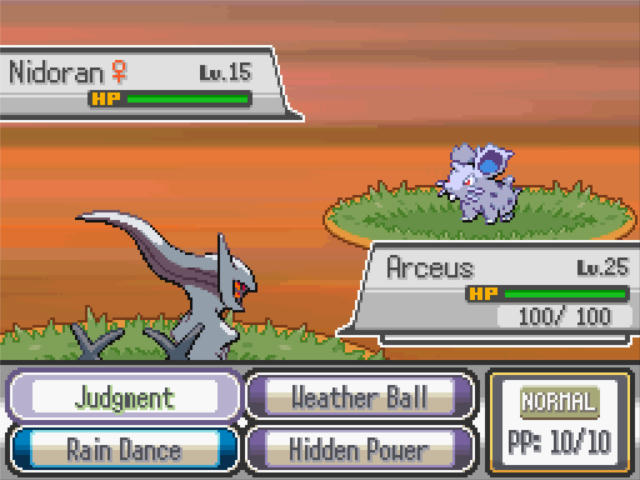
\includegraphics[width=0.5\textwidth]{figures/combat.jpg}
        \caption{Jugador eligiendo el ataque de su pokémon.}
        \label{fig:turn}
\end{figure}

\section{Pokémons}
Las batallas se realizan entre pokémons, en la actualidad existen 1025 especies de pokémons. Nosotros trabajaremos con una muestra reducida para facilitar el entrenamiento de la red neuronal.

\begin{figure}[H]
	\centering
	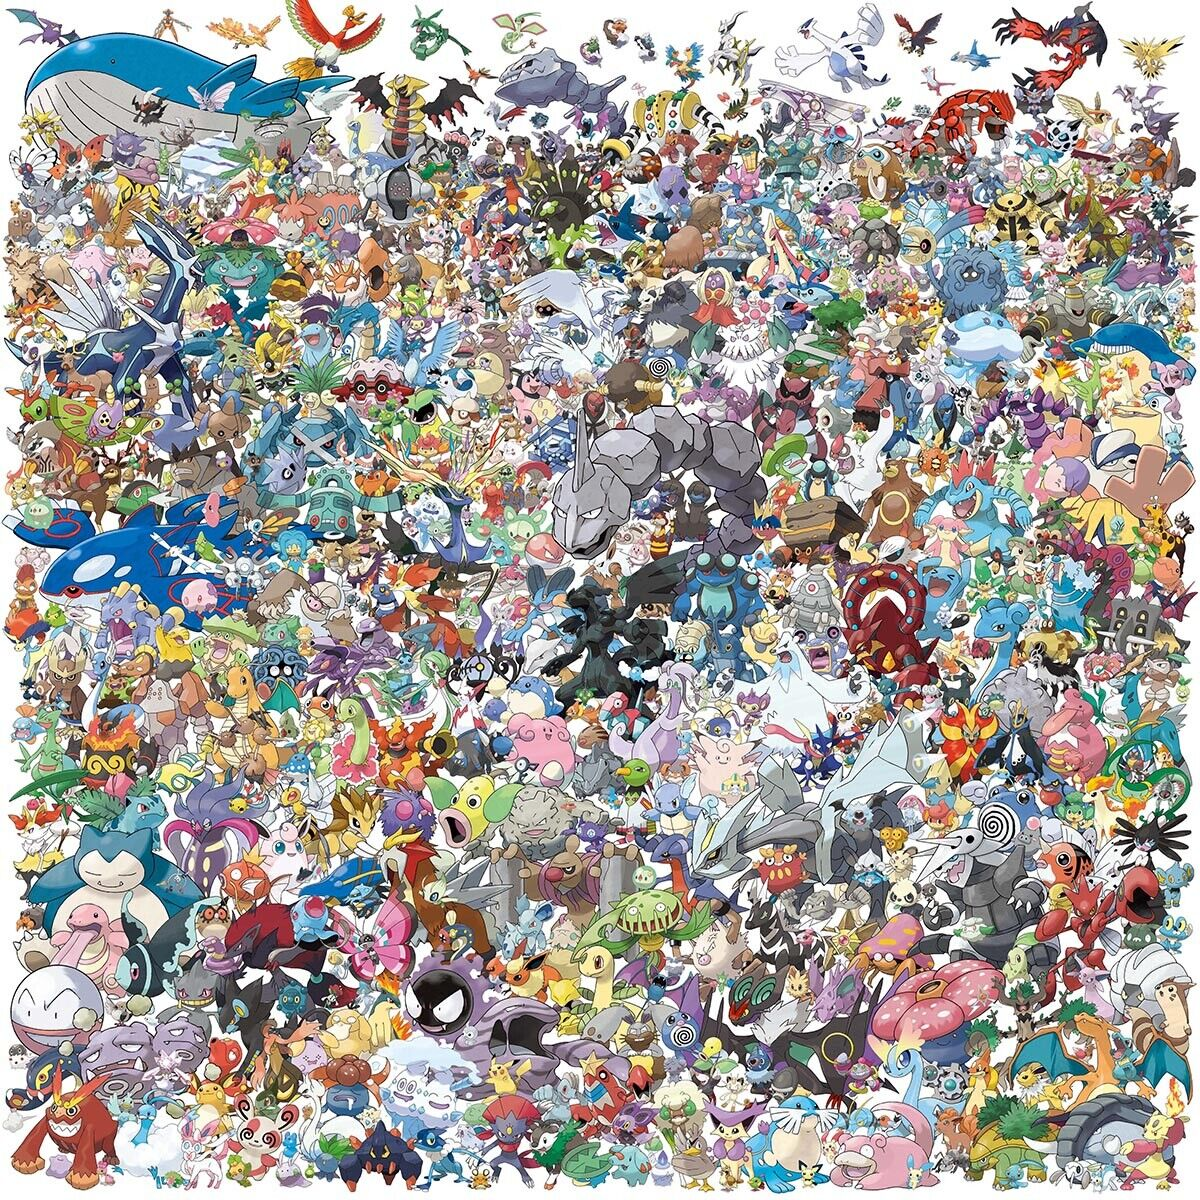
\includegraphics[width=0.5\textwidth]{figures/pokemons.jpg}
	\caption{Algunos de los pokémons.}
	\label{fig:pokemon}
\end{figure}

\section{Tipos}
Cada pokémon tiene un tipo, existen 18 tipos diferentes, cada tipo tiene una serie de debilidades y fortalezas contra otros tipos. Además del tipo los pokémons tienen otras estadísticas como los puntos de vida, ataque, defensa o velocidad. 

\begin{figure}[H]
	\centering
	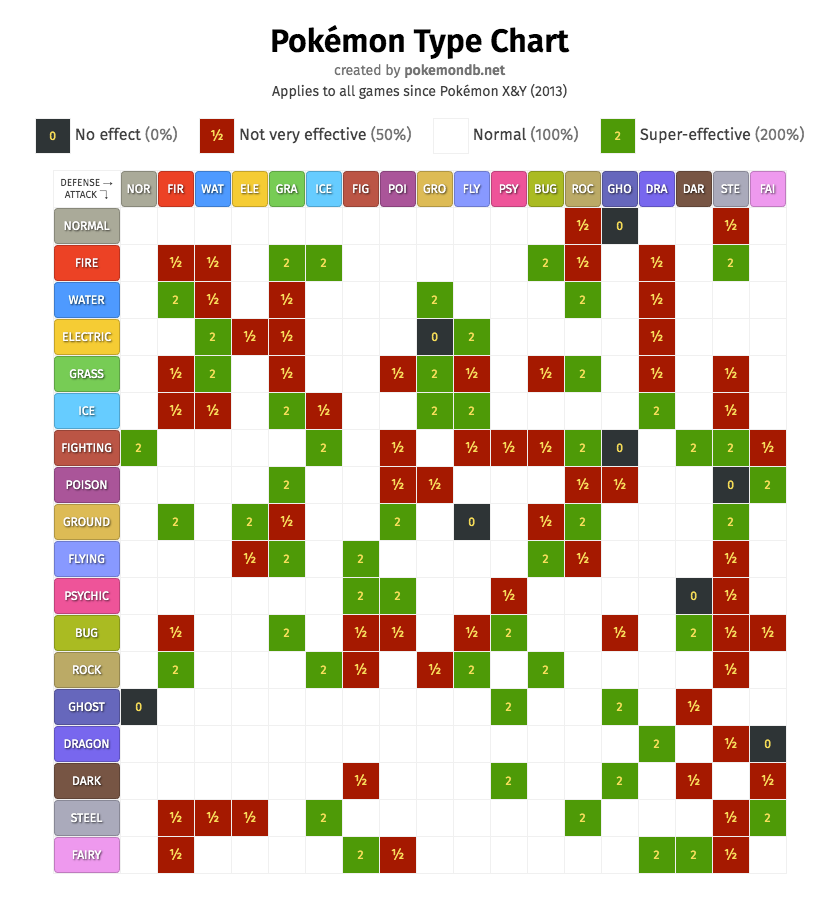
\includegraphics[width=0.5\textwidth]{figures/chart.png}
	\caption{Tabla de tipos.}
	\label{fig:types}
\end{figure}

\section{Movimientos}
Cada pokémon tiene una serie de movimientos, los cuales realizan una acción en la batalla, ya sea atacar, curar, aumentar la defensa, etc. Cada movimiento tiene un tipo, una potencia y una precisión. El tipo determina contra que pokémons es eficaz el ataque, la potencia influye en el daño del ataque y la precisión determina la probabilidad de acierto (que en nuestro caso siempre será 100\%). A día de hoy existen 934 movimientos, la mayoría consisten en atacar pero hay algunas excepciones.

\begin{figure}[H]
	\centering
	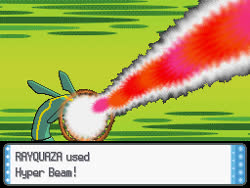
\includegraphics[width=0.5\textwidth]{figures/hiperrayo.jpg}
	\caption{Un pokémon usando el movimiento hiperrayo.}
	\label{fig:hiperrayo}
\end{figure}
